\chapter{Energiekalibrierung des Spektrometers}
\section{Theoretische Grundlagen}
Die Energiekalibrierung eines Gammaspektrometers basiert auf der Zuordnung von Kanalnummern eines Multikanalanalysators (MCA) zu bekannten $\gamma$-Übergangsenergien. Hierfür werden Proben mit bekannten Zerfallsprofilen und spektraler Vielfalt verwendet. Der $^{152}$Eu-Kern eignet sich besonders gut für die Kalibrierung im Energiebereich zwischen etwa 100 keV und 1,4 MeV, da er eine große Anzahl von Gamma-Übergängen enthält. Zusätzlich wird der 662-keV-Übergang von $^{137}$Cs verwendet, um die Kalibrierung im mittleren Energiebereich zu stabilisieren.
\paragraph{$\gamma$-Spektrum von $^{152}$Eu}
Der Zerfall von $^{152}$Eu führt über mehrere angeregte Zustände des $^{152}$Sm zu einer Vielzahl charakteristischer $\gamma$-Linien.\\
\begin{table}[htbp]
    \centering
    \begin{tabular}{c|c|c}
        \textbf{Energie (keV)} & \textbf{Intensität (\%)} & \textbf{Übergang} \\
        \hline
        $121,7817\pm0,0003 $ & $28,53 \pm 0,16$ & $^{152}$Eu $\rightarrow$ $^{152}$Sm \\
        $244,6974 \pm 0,0008 $ & $7,55 \pm 0,04$ & $^{152}$Eu $\rightarrow$ $^{152}$Sm \\
        $344,2785 \pm 0,0012 $ & $26,59 \pm 0,20$ & $^{152}$Eu $\rightarrow$ $^{152}$Gd \\
        $411,1165 \pm 0,0012 $ & $2,237 \pm 0,013$ & $^{152}$Eu $\rightarrow$ $^{152}$Gd \\
        $443,9606 \pm 0,0016 $ & $2,827 \pm 0,014$ & $^{152}$Eu $\rightarrow$ $^{152}$Sm \\
        $778,9045 \pm 0,0024 $ & $12,93 \pm 0,08$ & $^{152}$Eu $\rightarrow$ $^{152}$Gd \\
        $867,380 \pm 0,003 $ & $4,23 \pm 0,03$ & $^{152}$Eu $\rightarrow$ $^{152}$Sm \\
        $964,057 \pm 0,005$&$14,51 \pm 0,07$&$^{152}$Eu $\rightarrow$ $^{152}$Sm\\
    \end{tabular}
    \caption{Auswahl der häufgisten $\gamma$-Übergänge von $^{152}$Eu mit ihren Energien und Intensitäten.\cite{Eu-peaks}}
    \label{tab:europium_lines}
    \end{table}

Diese Linien dienen als Referenzpunkte für die Kalibrierung des Spektrometers.
Aufgrund der begrenzten Energieauflösung des Detektors können sich mehrere nahe beieinander liegende Übergänge überlappen und einen einzigen Peak bilden. 
Diese Überlappung tritt besonders häufig bei Spannungen über 400 keV auf, da der Linienabstand dann kleiner als die Halbwertsbreite (FWHM) des Detektors ist.
Zur genauen Identifizierung der Linien wird eine Hintergrundmessung ohne Probe durchgeführt und anschließend vom Spektrum subtrahiert, um die Auswirkungen von Umgebungsstrahlung und elektrischem Rauschen zu eliminieren.
\paragraph{Lineare Energiekalibrierung}
Die Beziehung zwischen der Kanalnummer $K$ und der Energie $E$ eines $\gamma$-Übergangs wird durch eine lineare Funktion beschrieben:
\begin{align}
    E(K) = aK + b
    \label{Gl:kalibrierung}
\end{align}
Die Parameter $a$ und $b$ werden durch eine lineare Regression der bekannten Energien der $^{152}$Eu-Übergänge gegen die gemessenen Kanalnummer bestimmt. \\
Dazu wird noch der $^{137}$Cs-Peak verwendet, um die Kalibrierung im mittleren Energiebereich zu stabilisieren und systematische Unsicherheiten zu reduzieren.
\paragraph{Detektoreffizienz}
Die Wahrscheinlichkeit, dass ein $\gamma$-Photon mit der Energie $E$ im Detektor ein vollständiges Signal erzeugt, wird mit der Detektoreffizienz $\epsilon(E)$ beschrieben. Diese hängt von der gemessenen Peakfläche $A(E)$, der Anzahl der emittierten $\gamma$-Photonen $N_\gamma(E)$ und der Messzeit $t$ ab:
\begin{align*}  \epsilon(E) = \frac{A(E)}{N_\gamma(E) \cdot t}  \end{align*}
Die absolute Aktivität der Probe ist unbekannt, also kann nur die relative Effizienz bestimmt werden. Aber das ist für die Energieabhängigkeit der Effizienz ausreichend, denn der unbekannte Proportionalitätsfaktor ist für alle Energien der gleiche und fällt beim Normalisieren während der Analyse weg.\\
Im üblichen Fall fällt die Detektoreffizienz mit steigender Energie ab, denn hochenergetische $\gamma$-Photonen haben eine geringere Wahrscheinlichkeit, vollständig im Detektor absorbiert zu werden. 
Daher ist es wichtig, die Effizienzkurve über den gesamten Energiebereich zu bestimmen, um die gemessenen Spektren korrekt interpretieren zu können.
\section{Durchführung}
Zunächst wird der Detektor in einem Winkel von 90° ausgerichtet, sodass er direkt auf die Probenhalterung zeigt. 
Während dieses Vorgangs bleibt die Cäsiums-Quelle geschlossen; die Europiumquelle mit geringer Aktivität wird an die Targethalterung angebracht.
Mit dieser Versuchsanordnung soll der Einfluss der Hintergrundstrahlung der Cäsium-Quelle auf die Messung minimieren werden.

Die Messungen wurden mit einer Totzeit von 300 s durchgeführt (mit als auch ohne die Europiumquelle). 
Das resultierende Hintergrundspektrum wurde dazu verwendet, den dem Cäsium zuzuschreibenden Hintergrund zu eliminieren.
\section{Auswertung}
Die gemessenen Spektren werden mittels eines Peak-Fitting-Algorithmus gefittet, um die den Peaks entsprechenden Kanalnummern zu ermitteln. Anschließend werden die bekannten Intensitäten der modifizierten $^{152}$Eu-Probe mit den gemessenen Kanalnummern verglichen, um die Kalibrierungsparameter $a$ und $b$ zu bestimmen. 
Die Energieeffizienz des Detektors wurde durch den Vergleich des gemessenen Bereichs mit dem Referenzwert evaluiert, wobei die Probeneigenschaften sowie die Messdauer berücksichtigt wurden. 
Die Ergebnisse werden in Form von Kalibrierungskurven und Effizienzgrafiken dargestellt, um die Robustheit des Detektors zu veranschaulichen.\\
\begin{figure}[htbp]
    \centering
    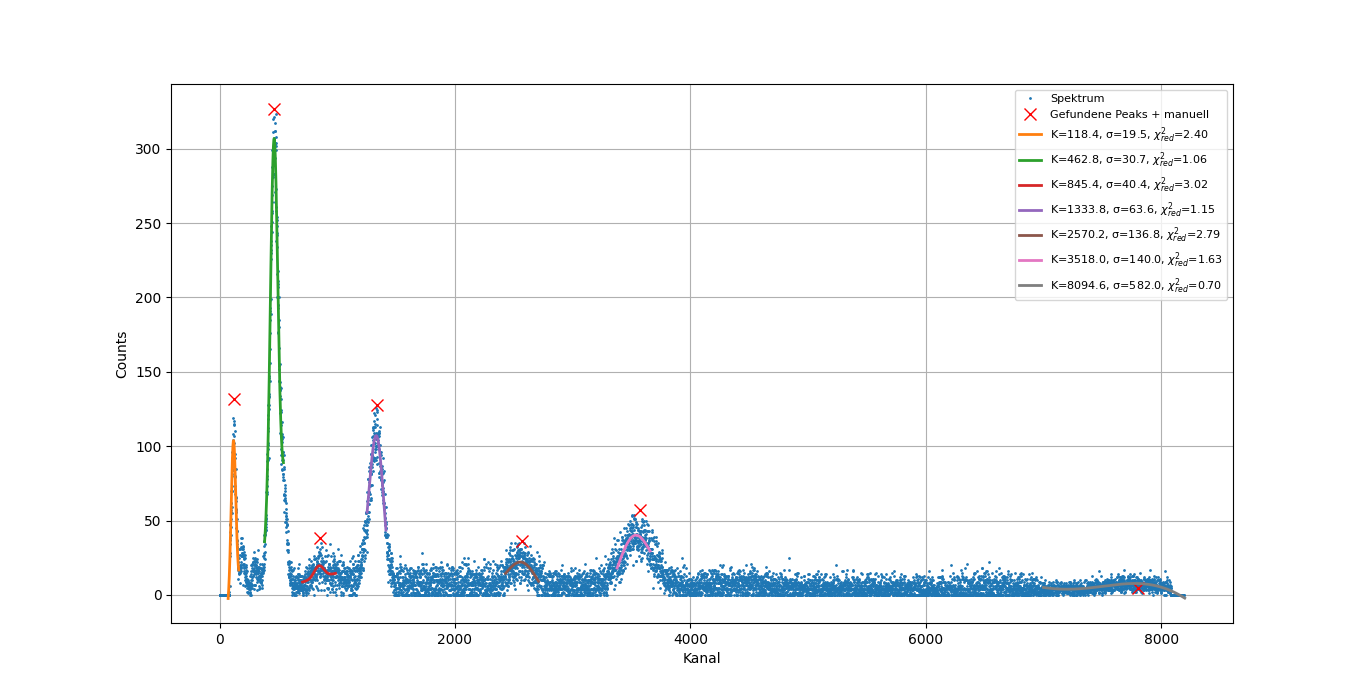
\includegraphics[width=0.75\textwidth]{figs/Europiumfinal.png}
    \caption{Frontales Kalibrations-Spektrum der $^{152}$Eu-Quelle.}
    \label{plot:plot1}
\end{figure}
%\FloatBarrier
Abbildung \ref{plot:plot1} zeigt mehrere Emissionslinien, von denen 4 eindeutig identifiziert werden können:
\begin{table}[htbp]
    \centering
    \begin{tabular}{|c|c|c|}
        \hline
        Kanalzentrum&Energie (keV)&$^{152}$Eu-Linie\\
        \hline
        118&0,8&Untegrund\\
        463&34&Untergrund\\
        845&74&Untegrund\\
        1334&$(122,8\pm4,7)$&121,78 keV\\
        2570&$(245,5\pm0,8)$&244,70 keV\\
        3518&$(341,0\pm9,3)$&344,28 keV\\
        8095&$(800,0\pm20,2)$&778,90 keV\\
        \hline  
    \end{tabular}
    \caption{Tabelle der identifizierten Peaks im Spektrum der $^{152}$Eu-Quelle, die Unischerheiten wurden gemäß der Gaußschen Fehlerfortpflanzung berechnet.}
\end{table}\\\
 Der Ursprung dieser Linien wird aus dem $^{152}$Eu-Zerfallschema \ref{tab:europium_lines} sowie aus den Summenpeaks und charakteristischen Röntgenanregungen der Quelle abgeleitet. 
 Die drei Linien bei 0,8 keV, 34 keV und 74 keV können nicht den Emissionslinien von $^{152}$Eu zugeordnet werden, da sie außerhalb des Energiebereichs liegen, in dem die Übergänge vom Europium auftreten. 
 Die Fehlerfortpflanzung bei diesen Linien führt zu großen relativen Unsicherheiten, die physikalisch nicht sinnvoll interpretierbar sind und wurden daher nicht angegeben.
 Diese Linien entstehen vermutlich von der Röntgen-Absorbtionskanten von Xenon, welches Bestandteil der Umgebungsluft ist, wobei die K-Kante dem 34,56 keV Übergang entspricht, sowie Eisen (L-Line $\sim$ 0,8)  und Blei (K-Linie $\sim$ 74,97) \cite{LBL_XrayData} welche vermutlich von der Abschirmung/dem Halter der Europiumquelle stammen, da die strahlung in alle Richtungen ausgeht. 
 Alle vier identifizierten Peaks liegen innerhalb ihrer Unsicherheiten im Bereich der Energien der $^{152}$Eu-Übergänge. 
 Dies bestätigt, dass die Kalibrierungspunkte korrekt zugeordnet wurden und dass die Messungen des Detektors im betrachteten Energiebereich zuverlässig sind.
\\
\begin{figure}[htbp]
    \centering
    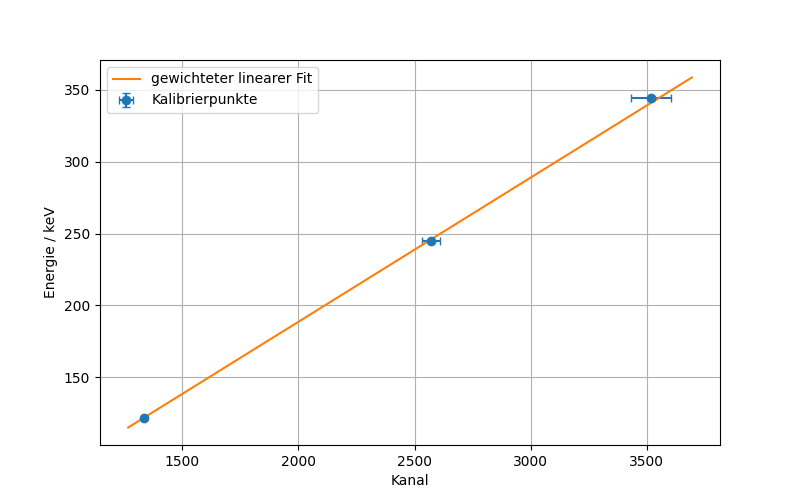
\includegraphics[width=0.75\textwidth]{figs/Kalibrierungfinal.png}
    \caption{Lineare Anpassung von Kanal-Index k des Peaks an die Energie E}
    \label{plot:plot2}
\end{figure}
%\FloatBarrier
Auf der Grundlage der Anpassungsgleichung für die Kanalenergie (Gleichung \ref{Gl:kalibrierung}) und der vorgeschlagenen linearen Bereiche (Tabelle \ref{tab:peakfits}) wurden die den Kanälen entsprechenden Energien in keV ermittelt, wie in Abbildung \ref{plot:plot2} dargestellt. 
Es wurden nur drei Peaks anstand von den vier identifizierten Peaks zur Kalibrierung verwendet, da der Peak eine recht größere Unsicherheit aufweist im vergleich zu den anderen Peaks und seine Amplitude so niedrig ist, dass beim man beim Fitten keine sinnvollen Kalibrierungsparameter erhalten konnte.
\begin{table}[htbp]
    \centering
    \begin{tabular}{c|c|c|c|c|c|c}
        Nr. & Kanalzentrum & Fehler & Höhe $A$ & $\sigma$ & $\chi^2$ & $\chi^2$ \\
        \hline
        1 & 118.37  & 0.93   & 103.78 & 19.51  & 206.06 & 2.40 \\
        2 & 462.84  & 0.44   & 252.81 & 30.72  & 165.00 & 1.06 \\
        3 & 845.45  & 6.19   & 8.08   & 40.40  & 833.85 & 3.02 \\
        4 & 1333.81 & 5.68   & 105.02 & 63.60  & 179.85 & 1.15 \\
        5 & 2570.24 & 37.35  & 24.84  & 136.77 & 770.62 & 2.79 \\
        6 & 3517.98 & 84.84  & 40.53  & 140.00 & 448.66 & 1.63 \\
        7 & 8094.63 & 290.90 & 44.42  & 581.98 & 721.00 & 0.70 \\
    \end{tabular}
    \caption{Gefittete Peaks mit Kanalzentrum, Unsicherheiten, Amplituden, Breiten und $\chi^2$-Parametern.}
    \label{tab:peakfits}
\end{table}
\newpage
Die Anpassungsparameter für die verwendete lineare Gleichung (Gleichung \ref{Gl:kalibrierung}) lauten wie folgt:
\begin{align*}
    &a = (0.100345 \pm 0.002457) \text{ keV/Kanal} \\
    &b = (-12.072 \pm 3.417) \text{ keV}
\end{align*}
Da der erhaltene Geradenfit einen negativen Achsenabschnitt aufweist, könnte dies auf systematische Fehler oder auf eine zu niedrige Anzahl von Kalibrierungspunkten zurückzuführen sein. 
Es ist möglich, dass die lineare Annahme nicht vollständig gerechtfertigt ist, insbesondere im unteren Energiebereich, wo die Detektorantwort möglicherweise nicht linear ist.
Dies könnte auch bedeuten, dass der MCA für niedrige Energien noch triggert, was erklären würde, dass 3 Peaks im Bereich bis 100 keV beobachtet werden, obwohl diese nicht den Emissionslinien von $^{152}$Eu zugeordnet werden können. 
Es ist auch möglich, dass der Hintergrund nicht substrahiert wurde, und dies könnte zu einer Verzehrung der Kalibrierung führen.\\ 
Weitere Messungen und zusätzliche Kalibrierungspunkte könnten sinnvoll sein, um die Genauigkeit der Kalibrierung zu verbessern und die Ursache für den negativen Achsenabschnitt zu identifizieren.\\

Um die nachfolgenden Messungen zu korrigieren, ist es nötig, die Detektoreffizienz $\epsilon(E)$ in Abhängigkeit von der Kannalnummer zu bestimmen. 
Da das Szintillationsspektrometer sowohl bei niedrigen als auch bei hohen Energien eine geringe Nachweiswahrscheinlichkeit aufweist, ist zu erwarten, dass die Effizienz jenseits des optimalen Arbeitsbereichs des verwendeten NaI(Tl)-Kristalls signifikant abfällt.\\
Ohne Kenntnis der Aktivität der Quelle, sowie der genauen Detektorgeometrie, kann die relative Effizienz dennoch durch die gemessene Intensität der Peaks ($I_{meas}\propto A$) im Vergleich zur Erwarteten Intensitäten der $^{152}$Eu-Übergänge ($I_{exp}$) bestimmt werden:
\begin{align*}
    \epsilon(E) \propto \frac{I_{meas}(E)}{I_{exp}(E)}\approx\frac{\epsilon(E)}{max(\epsilon(E))}
\end{align*}
Als empirische Fitfunktion für die Effizienzkurve wird eine Gaußfunktion der Form $\epsilon(E) = A \cdot E^b \cdot e^{-c \cdot E}$ verwendet, wobei a,b und c Fitparameter sind, die durch eine nichtlineare Regression bestimmt werden. Abbildung \ref{plot:plot3} zeigt die gemessene Effizienzkurve mit der angepassten Fitfunktion.\\
Man erhält folgende Fitparameter:
\begin{align*}
    &a = (7.341479\cdot10^{-11} \pm 1.013317\cdot10^{-09})\\
    &b = (3.615230 \pm 2.091268)\\
    &c = (2.008950\cdot10^{-03} \pm 9.523332\cdot10^{-04})\\
\end{align*}
\begin{figure}[htbp]
    \centering
    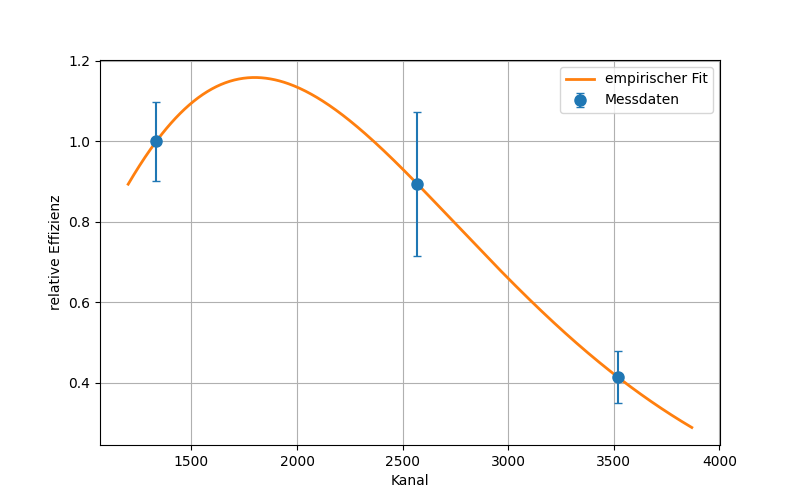
\includegraphics[width=0.75\textwidth]{figs/Effizienzfinal.png}
    \caption{Lineare Anpassung von Kanal-Index k des Peaks an die Energie E}
    \label{plot:plot3}
\end{figure}
\FloatBarrier
 Die Fitfunktion entspricht den erwarteten exponentiellen Abfall der Effizienz mit steigender Energie bei Szintillationsdetektoren.\\
 Dennoch ist aufgrund der begrenzten Datenmenge entspricht die gefittete Kurve nur annähernd der Effizienz. 
 Man erhält $\chi^2=0$, was durch eine Überanpassung entstanden sein kann, da die Anzahl an Fitparametern gleich der Anzahl an Messpunkten ist, was zu hoch ist und zu einer perfekten Anpassung führt. Zudem ist eine Anpassung auf drei Datenpunkten leider nicht sehr aussagekräftig.\\
 Wenngleich die verwendete empirische Anpassung die geschätzten Daten widerspiegelt, ist sie nicht eindeutig durch die gemessenen Daten bestimmt und sollte insbesondere außerhalb des gemessenen Bereichs nicht überinterpretiert werden. 
 Für präzisere Vorhersagen ist genaueres Effizienzmodell erforderlich, sowie eine größere Menge an Datenpunkten zum fitten.
